\section{Additional Experimental Results}
\label{app:additional}
\paragraph{Additional Experimental Details} Experiments on nonlinear networks were carried out using an A6000. All other experiments were run locally on CPU. Experiments on nonlinear networks are based on code from \url{https://github.com/locuslab/edge-of-stability}~\citep{cohen2021stability}.

\subsection{Is Linear Warmup Necessary?}
\label{app:warmup-necessity}
\begin{figure}[!t]
    \centering
    \subfigure[Step warmup.]{
        \includegraphics[width=0.45\linewidth]{figures/step-warmup/lr0.0023_Twarmup10000_alpha0.2/u2-v2_hess-sharpness.pdf}
        \label{fig:ldn-step-warmup}
    }
    \subfigure[Terminating the warmup.]{
        \includegraphics[width=0.45\linewidth]{figures/warmup_stop/lr0.005_Twarmup5000_Twarmupstop2150_alpha0.2/u2-v2_hess-sharpness.pdf}
        \label{fig:warmup-stop}
    }
    \caption{Ablations on the learning rate warmup. (a) Step warmup is used instead of linear warmup. (b) The warmup period is initially set to $5000$ iterations, but the warmup is terminated at iteration $2150$ around the iteration where the sharpness crosses the MSS.}
    \label{fig:ldn-warmup}
\end{figure}

Although we use linear warmup in our experiments, we emphasize that linear warmup is {\it not} necessary to induce the catapults.
As mentioned in the main text, we observe that the main criteria for inducing the catapults are (1) for the iterates to be in a neighborhood of a stable minimum and (2) for the current learning rate to be large enough that the minimum is unstable (in that the sharpness of the minimum is above the MSS) but not so unstable that training diverges.
% and are (1) convergence to an initial (sharp) minimum and (2)
Linear warmup satisfies these two criteria by (1) stably moving the iterates towards a minimum under a low learning rate and (2) automatically finding a suitably large learning rate (that does not lead to divergence) by gradually increasing the learning rate. However, as long as the two criteria are met, catapults can be induced without linear warmup.

\paragraph{Other Warmup in the LDN.}
To show that the specific form of the warmup is not essential in inducing the catapults, we train an LDN using a step warmup scheduler.
We use the learning rate of $10^{-5}$ for the first $10000$ iterations and then $0.0023$ for the remaining $10000$ iterations. Here, it is necessary to use a sufficiently long warmup period to ensure that the pre-catapult training loss is close to zero. 
% Note that under the same learning rate, the MSS of GD and PHB differ by a factor of $(1+\beta)$.
%Since both GD and PHB are initialized at the same $\alpha \cdot \bm{1}$, the learning rate used for the PHB experiment is the specified learning rate multiplied by $(1+\beta)$ to match the MSS and ensures that if the sharpness hits the MSS for GD, it also hits the MSS for PHB.
As shown in Figure~\ref{fig:ldn-step-warmup}, this setting also induces a catapult despite not using linear warmup.
It should be noted that, unlike linear warmups, the final learning rate must be carefully tuned to prevent training from diverging. 
%We can interpret step warmup as a two-phase process of (1) finding a stable minimum by training under low $\eta$ and then (2) inducing a catapult by using a constant but sufficiently large $\eta$.
%{\color{red}Notably, this suggests that if the parameters are initialized close to a minimum and $\eta$ is initialized so that the initial sharpness is only slightly above the MSS, large catapults can be induced while keeping $\eta$ constant as in the second phase of step warmup. Based on this observation, we consider a constant (but large) $\eta$ setting to simplify the analysis in Section \ref{sec:prolong}.}
% (unlike linear warmup, which ``smoothly'' leads to a point that induces catapults): if the learning rate is too small, the catapult is not induced, and if it is too large, training diverges.

To show the effectiveness of the linear warmup in finding the appropriate scale of the learning rate for inducing catapults, we terminate the warmup as soon as the sharpness crosses the MSS, even before the prescribed warmup period ends.
As shown in Figure \ref{fig:warmup-stop}, this is enough to induce catapults for PHB, supporting our claim that linear warmup has the advantage of ``smoothly'' finding a suitable learning rate for inducing catapults.

\paragraph{Linear Warmup in the Toy Model.}
Conversely, although we use a fixed learning rate for the toy model, we show in Figure~\ref{fig:toy-model-warmup} that catapults still occur even when using linear warmup.

\begin{figure}[!h]
    \centering
    \includegraphics[width=0.7\textwidth]{figures/scalar-net/warmup_scalar_trajectory_sharpness.pdf}
    \caption{Training the toy model using linear learning rate warmup still induces a catapult}
    \label{fig:toy-model-warmup}
\end{figure}


\subsection{Effects of ``Overshooting'' by Larger Catapults}
\label{app:overshooting}
When the momentum parameter $\beta$ is large, and an even larger catapult can happen and PHB may carry the iterates farther than the flattest minima, resulting in ``overshooting.''
% and a lesser degree of sharpness reduction. 
A good example can be found in the simple LDN loss $\gL(u,v) = \frac{1}{2}(u^2-v^2-1)^2$. As shown in Figure~\ref{subfig:ldn-overshooting}, momentum with $\beta = 0.99$ causes the iterates to move past the flattest minima $(u,v)=(1,0)$ and converge at a sharper solution. Overshooting may also explain why the final sharpness increases again in Figure~\ref{fig:LDN-main-phb} as $\alpha$ increases further: there is some optimal $\alpha$ for which momentum allows the iterate to reach the flattest possible minima, but increasing $\alpha$ even further may result in overshooting.

\begin{figure}[!h]
    \centering
    \subfigure[Theoretical lower bound on sharpness reduction based on toy example theory. At $\beta=0.99$, $\Delta S$ slightly decreases due to overshooting.]{
        \includegraphics[width=0.35\textwidth]{figures/ldn/ldn-2d-ub.pdf}
        \label{subfig:ldn-ub-bound}
    }
    \hfill
    \subfigure[Trajectory plot for $\beta=0.99$. The iterates overshoot past $(u,v)=(1,0)$ which is the flattest minima.]{
        \includegraphics[width=0.25\textwidth]{figures/ldn/ldn-2d-traj-0.99.pdf}
        \label{subfig:ldn-overshooting}
    }
    \hfill
    \subfigure[In the {\bf ReLU Scalar Network}, overshooting cause by momentum can lead to the neuron dying.]{
        \includegraphics[width=0.25\textwidth]{figures/scalar-net/scalar-overshoot.pdf}
        \label{subfig:scalar-overshooting}
    }
    \caption{Overshooting in simple models}
    \label{fig:simple-overshooting}
\end{figure}

% \subsection{Large Catapults Lead to More Dead Neurons}
% \label{app:dead}
As the loss landscape and manifold of minima become increasingly complex, overshooting may result in different outcomes, depending on the architectures. 
Another effect of overshooting relates to the lack of progressive sharpening in some of the experiments. 
In some of our experiments (Figures~\ref{fig:cifar10-exp}(a) and \ref{fig:cifar10-exp}(b)), we observed an interesting phenomenon where PHB does not display progressive sharpening after a few large catapults.
We conjecture this lack of progressive sharpening to be a result of large catapult inducing more dead neurons. Indeed, through a synthetic experiment with ReLU FCN, we show that large catapults due to PHB induce more dead neurons than GD; see Figure~\ref{fig:deadrelu}. Although seemingly unrelated, overshooting is one possible explanation as to why momentum induces more dead neurons. To illustrate this point, consider the case of the ReLU scalar network in Figure~\ref{subfig:scalar-overshooting}. Under certain settings, momentum can cause the iterates to overshoot the flattest possible minima $(u=0)$ and land in the region $u < 0$ which kills the ReLU neuron. A similar phenomenon could occur in more realistic networks as well.
\begin{figure}[!ht]
    \centering
    \subfigure[Sharpness.]{
        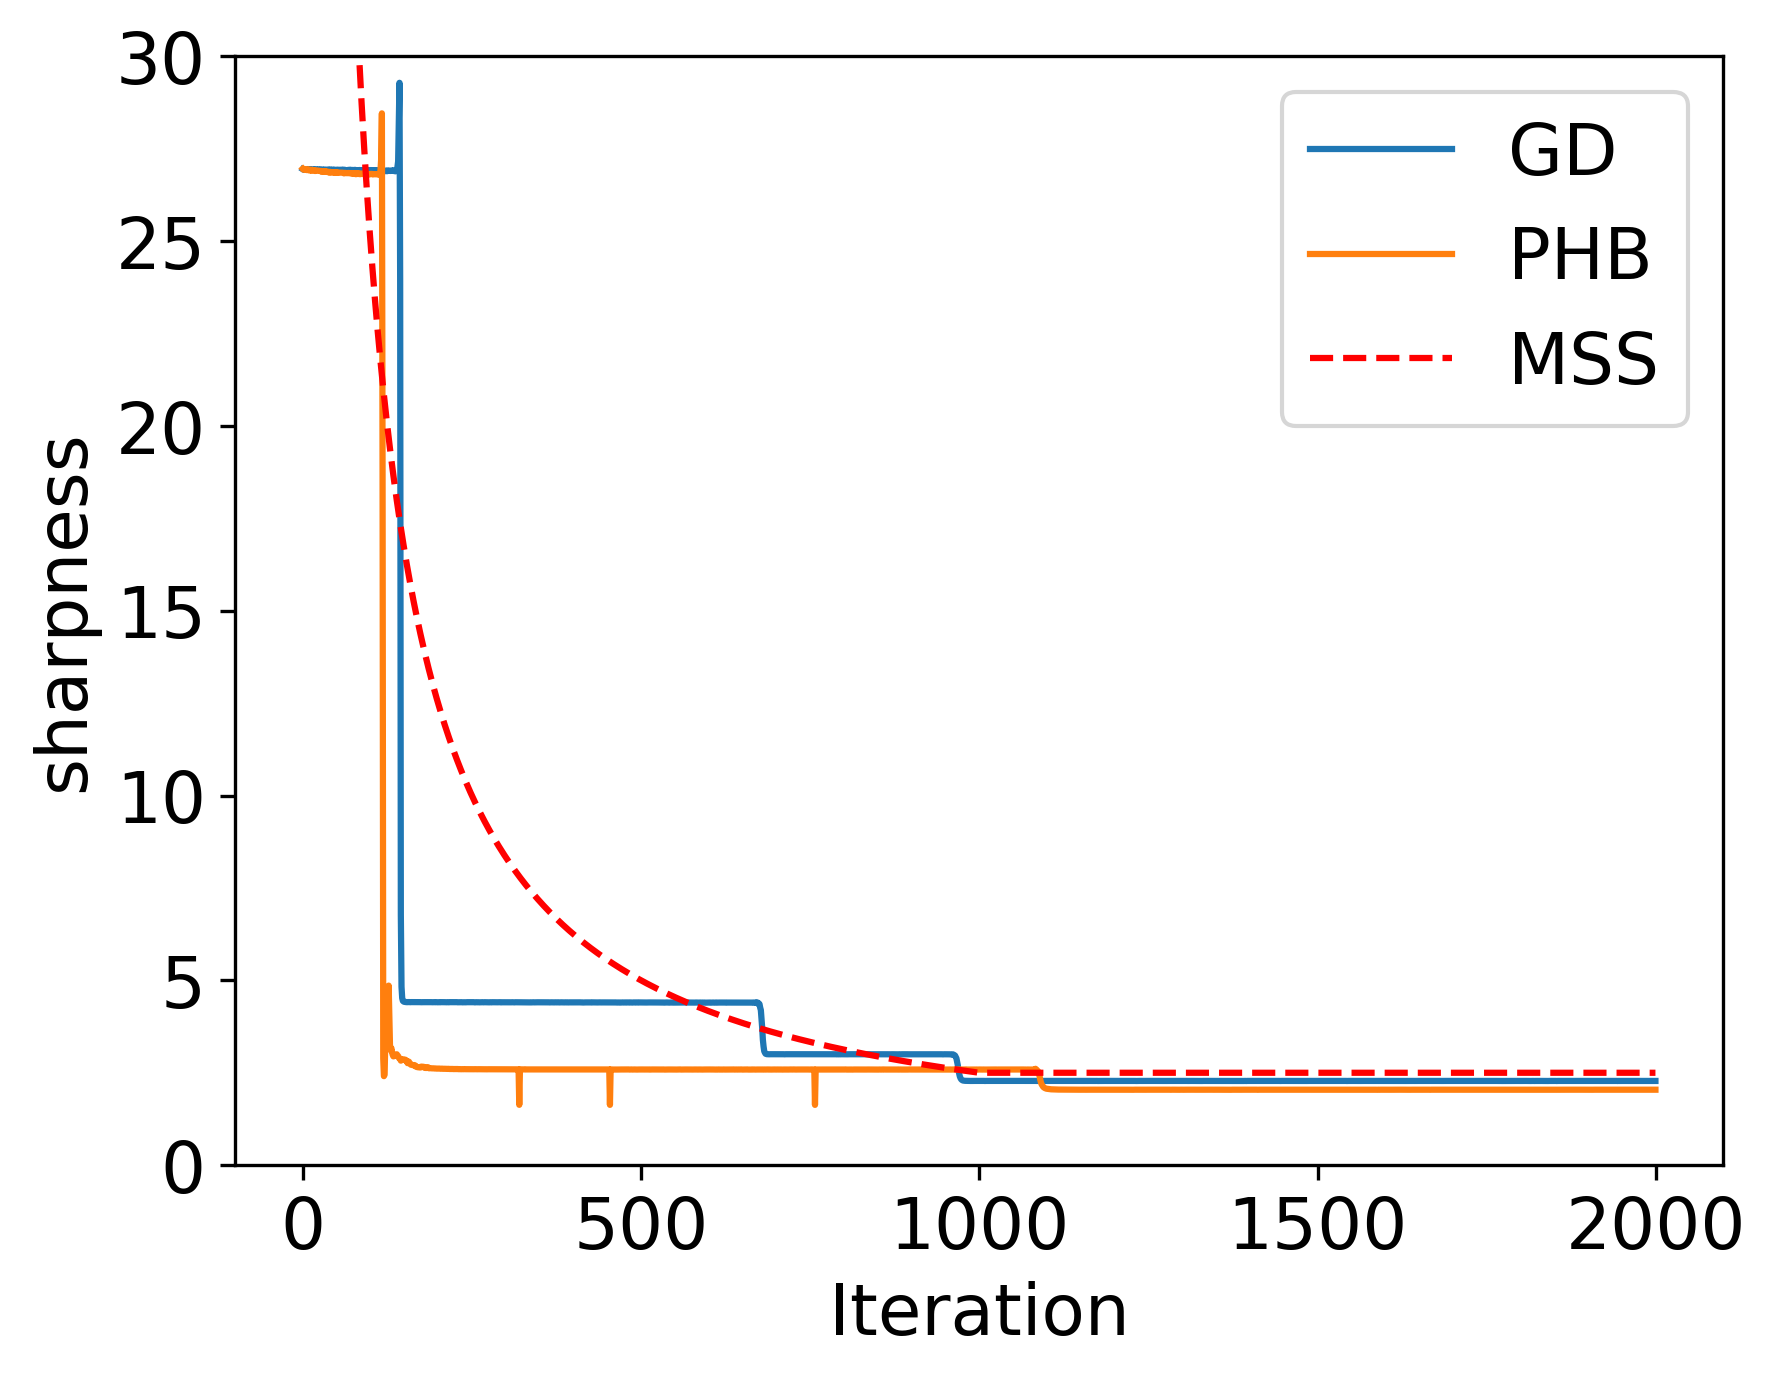
\includegraphics[width=0.46\linewidth]{figures/deadrelu_sharpness.png}
        \label{fig:deadrelu-sharpness}
    }
    \subfigure[Number of active neurons.]{
        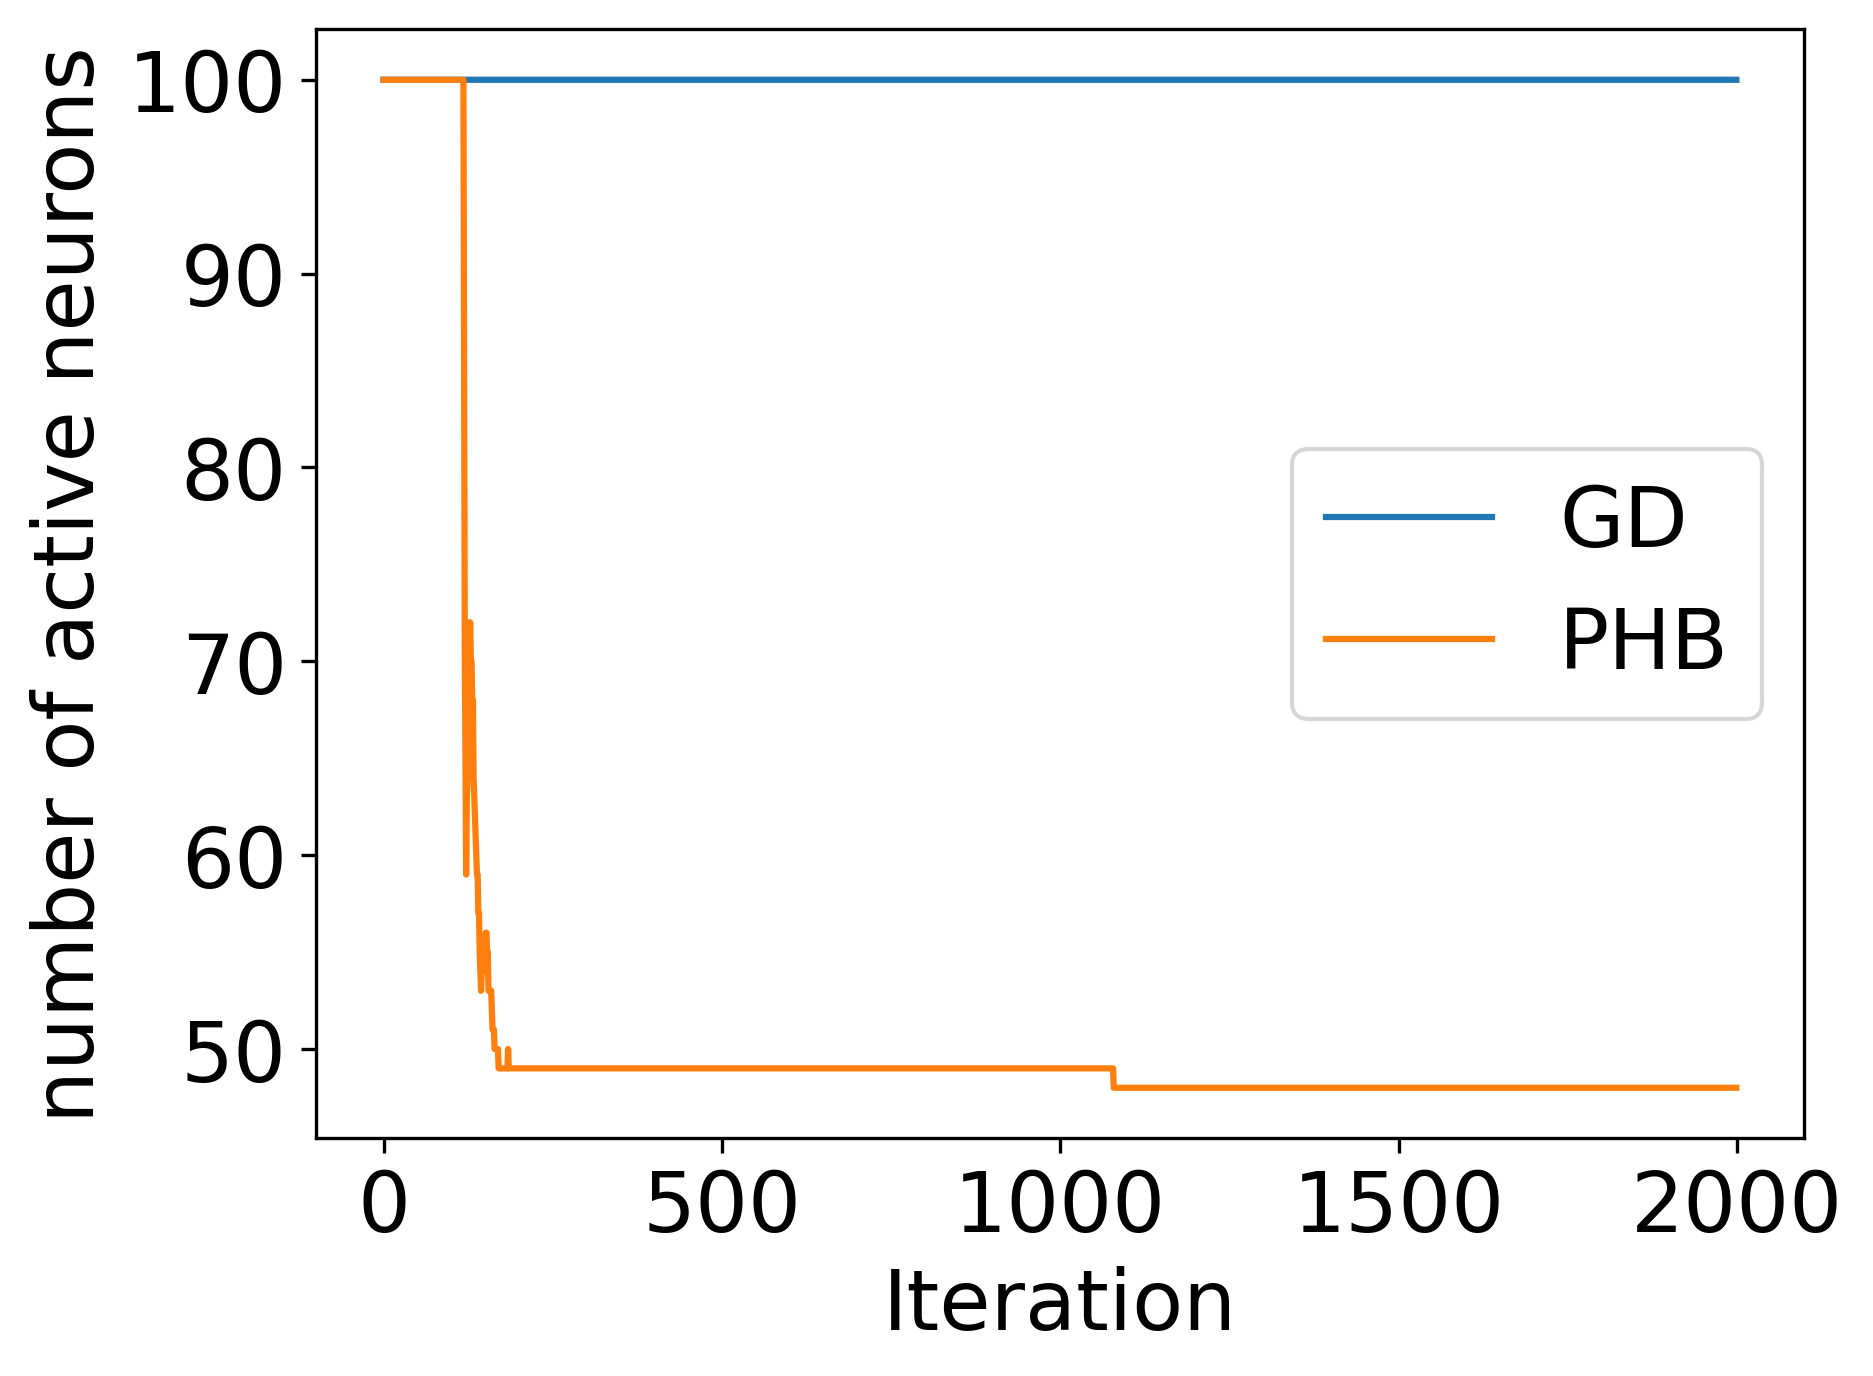
\includegraphics[width=0.46\linewidth]{figures/deadrelu_neurons.png}
        \label{fig:deadrelu-neurons}
    }
    \caption{2-layer FCN of width $100$ trained with MSE loss and rank-2 synthetic dataset~\cite{zhu2023catapult}, generated as follows: $\{(\vx_i, y_i)\}_{i=1}^{100}$ with $\vx_i \sim \gN_3(\vzero, \mI)$ and $y_i = (\vx_i)_1 (\vx_i)_2$.}
    \label{fig:deadrelu}
\end{figure}








% \subsection{Toy Example}
% \paragraph{Toy Example.}
% \label{sec:toy-example}
% To investigate the mechanism behind this phenomenon, we consider an elementary toy loss function, $f(x, y) = \frac{x^2}{2y}$, restricted to $y > 0$.
% Note that the (only) manifold of global minima is $x = 0$, and the sharpness decreases as $y$ increases in the $y > 0$ range. Figure~\ref{fig:toy} provides the trajectory plot for GD and PHB as well as the evolution of sharpness along with the MSS for a specific learning rate setup that induces catapult(s) for {\it both} GD and PHB.
% As with the LDN, GD goes through step-wise decreases in sharpness, whereas PHB goes through a single steep sharpness drop. One noteworthy observation is the diverging dynamics in the x-direction (which roughly coincides with the leading eigendirection close to the minima). Note also that the x-direction is orthogonal to both the manifold of global minima and the direction of sharpness decrease (positive y-direction). As such, the sharpness drops occur due to moving in the positive y-direction \emph{while} diverging in the x-direction.
% In the later stage, the dynamics in the x-direction undergoes damped oscillation due to reduced sharpness at larger $y$, stabilizing and forcing the dynamics to converge.
% % Appendix~\ref{app:toy-theory} provides additional experimental results and some theoretical intuitions on the effect of momentum.
% \begin{remark}
%     Here, we provide some justifications on the choice of our toy loss function.
%     The fact that $f$ has a manifold of global minima is consistent with assumptions used in prior works for analyzing gradient-based methods seeking flatter minima~\citep{damian2021noise,arora2022stability}.
%     Also, the uniqueness of such manifold makes the overall analysis simple, since if there are multiple manifolds of minima, the trajectory of PHB may display chaotic\footnote{Intuitively, each manifold of minima induces a potential field, whose overlap is expected to be quite complex.} behaviors such as overshooting.
% \end{remark}

% Here, we provide additional results for the toy example, $f(x, y) = \frac{x^2}{2y}$, for varying the final learning rate $\eta_f \in \{10^1, 10^2, 10^3, 10^5, 10^{10}\}$.
% We set the initialization to be $(0.01, 1)$, $\eta_i = 2$, and $\beta = 0.9$ for PHB.
% We report the results in Figures~\ref{fig:toy-eta} and \ref{fig:toy-sharpness}.
% % -beta=0.99

% % \item Turning off the momentum in the x-axis leads to instability in the training trajectory in that the fluctuation in the x-axis increases significantly, and no damped oscillation is observed.
% % This matches the theoretical intuition presented in Appendix~\ref{app:toy-theory} and our hypothesis that the momentum amplified the self-stabilization effect, i.e., more stable.


% \begin{remark}
% \label{rmk:momentum}
%     The reason that we could consider such large learning rates for our specific toy model is that the gradient at $(x, y)$ is $\left( \frac{x}{y}, -\frac{x^2}{2y^2} \right)$, and thus at higher $y$, the magnitude of the gradient field gets smaller.
%     This deters the iterates from ever diverging, and we believe that in our example, the iterates always converge regardless of the initialization and learning rate.
%     However, as this is often not the case, we expect that the self-stabilization effect described in Appendix~\ref{app:self-stabilization} is critical in stabilizing the dynamics of PHB for realistic scenarios.
% \end{remark}

% \begin{figure}[!h]
% \centering
% \includegraphics[width=0.3\textwidth]{toy/toy-trajectory.pdf}
% \includegraphics[width=0.3\textwidth]{toy/toy-trajectory-1e1.pdf}
% \includegraphics[width=0.3\textwidth]{toy/toy-trajectory-1e2.pdf}
% \includegraphics[width=0.3\textwidth]{toy/toy-trajectory-1e3.pdf}
% \includegraphics[width=0.3\textwidth]{toy/toy-trajectory-1e5.pdf}
% \includegraphics[width=0.3\textwidth]{toy/toy-trajectory-1e10.pdf}
% \caption{Trajectories of GD and PHB for the toy example.}
% \label{fig:toy-eta}
% \end{figure}

% \begin{figure}[!h]
% \centering
% \includegraphics[width=0.3\textwidth]{toy/toy-sharpness.pdf}
% \includegraphics[width=0.3\textwidth]{toy/toy-sharpness-1e1.pdf}
% \includegraphics[width=0.3\textwidth]{toy/toy-sharpness-1e2.pdf}
% \includegraphics[width=0.3\textwidth]{toy/toy-sharpness-1e3.pdf}
% \includegraphics[width=0.3\textwidth]{toy/toy-sharpness-1e5.pdf}
% \includegraphics[width=0.3\textwidth]{toy/toy-sharpness-1e10.pdf}
% \caption{Sharpness plots of GD and PHB for the toy example.}
% \label{fig:toy-sharpness}
% \end{figure}



\subsection{More experiments on Nonlinear Neural Networks}
\label{app:modern}

\subsubsection{Additional FCN Experiments}
For the nonlinear neural network experiment in Figure~\ref{fig:rank2}, we follow the setting of \citet{zhu2023catapult}.
We train a fully-connected 3-layer ReLU network of width $64$ on the synthetic rank-2 dataset.
The synthetic rank-2 dataset is generated by i.i.d. sampling data $\pmb{x}_i \sim \mathcal{N}(\pmb{0}, \mI_{d})$ and generating outputs $y_i = \pmb{x}_i^{(1)} \pmb{x}_i^{(2)}$ (product of the first two coordinates of $\pmb{x}_i$).
A rank2-$D$-$N$ dataset refers to the synthetic rank-2 dataset generated using $d=D$ whose training set consists of $N$ data points; in our experiment, we used a rank2-400-200 dataset.
% For the second nonlinear experiment in Figure \ref{subfig:resnet20_cifar10-1k_10class}, we use a ResNet20 with a 1k-datapoint, 10-class subset of CIFAR10 (Figure~\ref{fig:resnet20_cifar-128-1k} shows the result for a 128-datapoint, 2-class subset of CIFAR10.)
For both experiments, we used a momentum rate of $\beta=0.9$ and MSE loss. \\
% We use a fully-connected 3-layer ReLU network with constant width and train on two datasets using MSE loss: (1)  and (2) a synthetic rank-2 dataset. The simplified CIFAR10 dataset contains 128 training images taken from only the first 2 classes of the full CIFAR10 dataset. The synthetic rank-2 dataset is generated by i.i.d. sampling data $\pmb{x}_i \sim \mathcal{N}(\pmb{0}, \mI_{d})$ and generating outputs $y_i = \pmb{x}_i^{(1)} \pmb{x}_i^{(2)}$ (product of the first two coordinates of $\pmb{x}_i$). In Figure~\ref{fig:rank2}, we used a rank2-400-200 dataset, meaning that we used $d=400$ and a training set with 200 data points. In general, a rank2-$D$-$N$ dataset refers to the synthetic rank-2 dataset generated using $d=D$ whose training set consists of $N$ data points. We used a momentum rate of $\beta=0.9$ for all experiments.

\begin{figure*}[!ht]
\centering
\includegraphics[width=0.31\textwidth]{figures/sec3_rank2_train_loss_lin.pdf}
\hfill
\includegraphics[width=0.31\textwidth]{figures/sec3_rank2_test_loss_lin.pdf}
\hfill
\includegraphics[width=0.3\textwidth]{figures/sec3_rank2_sharpness_lin.pdf}

% \subfigure[CIFAR10-128, width=$256$, $\eta_i = 0.01$, $\eta_f = 0.2$]{
% \includegraphics[width=0.32\textwidth]{figures/sec3_cifar10_train_loss_lin.pdf}
% \hfill
% \includegraphics[width=0.32\textwidth]{figures/sec3_cifar10_test_loss_lin.pdf}
% \hfill
% \includegraphics[width=0.32\textwidth]{figures/sec3_cifar10_sharpness_lin.pdf}
% \label{fig:sharpness}
% }

\caption{FCN trained on the Rank2-400-200 dataset, $\eta_i = 0.02$, $\eta_f = 0.6$.
% Experiments using a 3-layer FCN and a ResNet20, both trained using MSE loss. The purple-shaded region represents the prescribed learning rate warmup period.
}
\label{fig:rank2}
\end{figure*}

% \begin{figure}[!ht]
%     \centering
%     \subfigure[ResNet20 trained on a 2-class 128-datapoint subset of CIFAR10, $\eta_i=0.01$, $\eta_f=0.02$]{
%         \includegraphics[width=0.32\textwidth]{figures/resnet20/cifar10-128_2class/lr0.01-0.02_mse/train_loss_log.pdf}
%         \includegraphics[width=0.32\textwidth]{figures/resnet20/cifar10-128_2class/lr0.01-0.02_mse/test_loss_log.pdf}
%         \includegraphics[width=0.32\textwidth]{figures/resnet20/cifar10-128_2class/lr0.01-0.02_mse/sharpness.pdf}
%     }
%     \subfigure[ResNet20 trained on a 1k-datapoint subset of CIFAR10, $\eta_i = 0.05$, $\eta_f = 0.1$]{
%         \includegraphics[width=0.32\textwidth]{figures/resnet20/cifar10-1k_10class/lr0.05-0.1_mse/train_loss.pdf}
%         \includegraphics[width=0.32\textwidth]{figures/resnet20/cifar10-1k_10class/lr0.05-0.1_mse/test_loss.pdf}
%         \includegraphics[width=0.32\textwidth]{figures/resnet20/cifar10-1k_10class/lr0.05-0.1_mse/sharpness.pdf}
%         \label{subfig:resnet20_cifar10-1k_10class}
%     }
%     \caption{ResNet20 experiments on CIFAR10 with MSE loss}
%     \label{fig:resnet20_cifar_mse}
% \end{figure}


\subsubsection{ResNet20 Experiments}
In Figure~\ref{fig:resnet}, we provide additional experiments on deep neural networks using the ResNet20 architecture. We observe that large catapults also occur for ResNet20 as well. \\

\begin{figure*}[!ht]
    \subfigure[2-class 128 subset of CIFAR10, $\eta_i=0.01$, $\eta_f=0.02$]{
        \includegraphics[width=0.29\textwidth]{figures/resnet20/cifar10-128_2class/lr0.01-0.02_mse/sharpness.pdf}
    }
    \hfill
    \subfigure[1k subset of CIFAR10, $\eta_i=0.01$, $\eta_f=0.1$]{
        \includegraphics[width=0.31\textwidth]{figures/resnet20/cifar10-1k_10class/lr0.01-0.1_warmup5000/sharpness.pdf}
    } 
    \hfill
    \subfigure[5k subset of CIFAR10, $\eta_i=0.01$, $\eta_f=0.1$]{
        \includegraphics[width=0.31\textwidth]{figures/resnet20/cifar10-5k/lr0.01-0.1_warmup5000_beta0.9/sharpness.pdf}
    }
    \caption{Results for ResNet20. The shaded region is the linear warmup period. 
    }
    \label{fig:resnet}
\end{figure*}









\subsubsection{Cross-Entropy Loss Experiments}
\label{app:ce-exp}
We provide additional experiments showing that large catapults still occur for networks trained using cross-entropy loss. As shown in Figure~\ref{fig:ce-fcn}, for PHB, large catapults occur during early training for FCN trained using Tanh activation and cross-entropy loss. Due to using cross-entropy loss, the iterates also converge quickly to a minimum with near-zero sharpness after the catapult. \\ 

Furthermore, for PHB, the iterates quickly converge to a minimum with near-zero sharpness right after the large catapult whereas for GD the iterates do not immediately converge to a flat minimum after the catapult. Instead, the sharpness of GD iterates settles at the MSS after the catapult before slowly converging towards flatter minima as training progresses.
\begin{figure}[!h]
    \centering
    \includegraphics[width=0.5\textwidth]{figures/fc-tanh/cifar10-1k/ce_w100_lr0.001-0.4_warmup400/sharpness.pdf}
    \caption{FCN Experiments using \emph{cross-entropy loss} on CIFAR10-1k, with Tanh activation, width 100, $\eta_i=0.001$, $\eta_f=0.4$}
    \label{fig:ce-fcn}
\end{figure}


% \subsubsection{Ablation for Nonlinear Neural Networks: Pre-catapult Training Loss}
% We conduct ablation studies to show that the catapult effect is an inherent characteristic of momentum itself and not simply a byproduct of confounding variables such as the pre-catapult training loss. In Fig. \ref{fig:modern-arch-ablation}, we conduct the same experiments as in Section \ref{sec:modern-arch} but where the warmup period does not begin from the first iteration and may not necessarily be equal for GD and PHB. Looking at the log training loss plot, we note that the catapult occurs either when GD and PHB achieve similar training loss, or when PHB has higher training loss than GD. Thus we believe that the pre-catapult loss level does not matter when inducing catapults. 

% \begin{figure}[!h]
% \centering
% \subfigure[Rank 2, width=$64$, $\eta_i = 0.02$, $\eta_f = 0.6$]{
% \includegraphics[width=0.33\textwidth]{figures/ablation_rank2_train_loss_log_cons-lin-cons.pdf}
% \hfill
% \includegraphics[width=0.33\textwidth]{figures/ablation_rank2_test_loss_cons-lin-cons.pdf}
% \hfill
% \includegraphics[width=0.33\textwidth]{figures/ablation_rank2_sharpness_cons-lin-cons.pdf}
% }
% \subfigure[CIFAR10-128, width=$256$, $\eta_i = 0.01$, $\eta_f = 0.2$]{
% \includegraphics[width=0.33\textwidth]{figures/ablation_cifar10_train_loss_log_cons-lin-cons.pdf}
% \hfill
% \includegraphics[width=0.33\textwidth]{figures/ablation_cifar10_test_loss_cons-lin-cons.pdf}
% \hfill
% \includegraphics[width=0.33\textwidth]{figures/ablation_cifar10_sharpness_cons-lin-cons.pdf}
% }

% \caption{Experiments using a fully connected 3-layer ReLU network with constant width trained using MSE loss. The region represents the learning rate warmup period. We use different warmup periods for GD and PHB to ensure that PHB does not achieve significantly lower training loss than GD when the first catapult occurs. Note that we use a log scale for the training loss plots}
% \label{fig:modern-arch-ablation}
% \end{figure}



% {\color{red}\subsection{Learning Rate Warmup Ablations}}
% {\color{red}In Figure \ref{fig:ldn-step-warmup}, we train a linear diagonal network using a step warmup scheduler. We train the network using a learning rate of $10^{-5}$ for $1000$ iterations and train using a learning rate of $0.00225$ for another $1000$ iterations. As shown in the figure, this setting also induces a catapult despite learning rate warmup not being used. However, it should be noted that the second (larger) learning rate needs to be carefully tuned: too small and the catapult is not induced, but too large and training diverges.}

% \label{app:warmup-ablation}
% \begin{figure}[h]
%     \centering
%     \includegraphics[width=0.32\textwidth]{figures/step-warmup/lr0.00225_Twarmup1000_alpha_0.2/u^2-v^2_train-loss_zoomed.pdf}
%     \includegraphics[width=0.32\textwidth]{figures/step-warmup/lr0.00225_Twarmup1000_alpha_0.2/u^2-v^2_test-loss_zoomed.pdf}
%     \includegraphics[width=0.32\textwidth]{figures/step-warmup/lr0.00225_Twarmup1000_alpha_0.2/u^2-v^2_hess-sharpness.pdf}
%     \caption{Linear Diagonal Network trained using step warmup}
%     \label{fig:ldn-step-warmup}
% \end{figure}

% {\color{red}Next, we show that linear learning rate warmup is suitable for finding the right scale of learning rate for inducing the catapults. By gradually increasing the learning rate, warmup is able to find a sufficiently large learning rate that induces catapults but not one that is so large as to cause the parameters to diverge. In Figure \ref{fig:warmup-stop}, we repeat the LDN experiment but instead of running learning rate warmup for the typically number of iterations, we terminate learning rate warmup once the sharpness crosses the MSS. As shown in the figure, this is enough to induce catapults for momentum GD, supporting our claim that learning rate warmup has the advantage of finding suitable learning rate for inducing catapults.}
% \begin{figure}[ht]
%     \centering
%     \includegraphics[width=0.32\textwidth]{figures/warmup_stop/lr0.005_Twarmup5000_Twarmupstop2150_alpha0.2/u^2-v^2_train-loss_zoomed.pdf}
%     \includegraphics[width=0.32\textwidth]{figures/warmup_stop/lr0.005_Twarmup5000_Twarmupstop2150_alpha0.2/u^2-v^2_test-loss_zoomed.pdf}
%     \includegraphics[width=0.32\textwidth]{figures/warmup_stop/lr0.005_Twarmup5000_Twarmupstop2150_alpha0.2/u^2-v^2_hess-sharpness.pdf}
%     \caption{Linear Diagonal Network trained using learning rate warmup. The warmup period is initially set to 5000 iterations, but warmup is terminated at iteration 2150 around the iteration where the sharpness crosses the MSS.}
%     \label{fig:warmup-stop}
% \end{figure}


\newpage
\subsection{Additional Results for $\beta = 0.99$}
\label{app:099}
We redo experiments with $\beta = 0.99$.
Overall, the trend is the same, with the effect of momentum more amplified.
We provide the necessary details and some discussions for each experiment redone.

\subsubsection{Linear Diagonal Networks}
\label{app:beta=0.99-ldn}
Here, we redo the experiments of Section~\ref{sec:ldn} with $\beta = 0.99$, where the results are reported in Figure~\ref{fig:LDN-0.99}.
Note how we expanded the range of $\alpha$'s to see the effect of momentum, which seems to be a bit ``delayed''.
But, at the same time, there is little instability in the trend in that once the curve reaches zero test loss, it stays there; this is in contrast to our $\beta = 0.9$ experiment (Figure~\ref{fig:LDN-main-phb} of Section~\ref{sec:ldn}), where there were some instabilities over $\alpha$'s.


\begin{figure}[!ht]
\centering
\subfigure[PHB Test Loss]{
\includegraphics[width=0.31\textwidth]{LDN/phb_0.99_testloss_vs_alpha.pdf}
\label{fig:LDN-testloss-0.99}
}
\subfigure[PHB Sharpness]{
\includegraphics[width=0.31\textwidth]{LDN/lr0.0042_beta0.99_warmup4200_u2-v2_sharpness_v_alpha.pdf}
\label{fig:LDN-sharpness-0.99}
}
\subfigure[PHB Log Train Loss]{
\includegraphics[width=0.31\textwidth]{LDN/lr0.0042_beta0.99_alpha0.4_warmup4200_train-loss_log.pdf}
\label{fig:LDN-trainloss-0.99}
}

\caption{Recall from Section~\ref{sec:ldn} that ``$\ell_1$ baseline'' and ``$\ell_2$ baseline'' in Figure~\ref{fig:LDN-testloss-0.99} stand for the solution with the minimal $\ell_1$ norm and the solution with the minimal $\ell_2$ norm to the regression problem, respectively.}
\label{fig:LDN-0.99}
\end{figure}


% \subsubsection{Toy Example}
% Here, we provide additional results for the toy example with $\beta = 0.99$ for vanilla GD and vanilla PHB.
% The results are shown in Figures~\ref{fig:toy-eta-beta} and \ref{fig:toy-sharpness-beta}.

% \begin{figure}[!h]
% \centering
% \includegraphics[width=0.3\textwidth]{toy-beta=0.99/toy-trajectory-5.pdf}
% \includegraphics[width=0.3\textwidth]{toy-beta=0.99/toy-trajectory-1e1.pdf}
% \includegraphics[width=0.3\textwidth]{toy-beta=0.99/toy-trajectory-1e2.pdf}
% \includegraphics[width=0.3\textwidth]{toy-beta=0.99/toy-trajectory-1e3.pdf}
% \includegraphics[width=0.3\textwidth]{toy-beta=0.99/toy-trajectory-1e5.pdf}
% \includegraphics[width=0.3\textwidth]{toy-beta=0.99/toy-trajectory-1e10.pdf}
% \caption{Trajectories of GD and PHB for the toy example.}
% \label{fig:toy-eta-beta}
% \end{figure}

% \begin{figure}[!h]
% \centering
% \includegraphics[width=0.3\textwidth]{toy-beta=0.99/toy-sharpness-5.pdf}
% \includegraphics[width=0.3\textwidth]{toy-beta=0.99/toy-sharpness-1e1.pdf}
% \includegraphics[width=0.3\textwidth]{toy-beta=0.99/toy-sharpness-1e2.pdf}
% \includegraphics[width=0.3\textwidth]{toy-beta=0.99/toy-sharpness-1e3.pdf}
% \includegraphics[width=0.3\textwidth]{toy-beta=0.99/toy-sharpness-1e5.pdf}
% \includegraphics[width=0.3\textwidth]{toy-beta=0.99/toy-sharpness-1e10.pdf}
% \caption{Sharpness plots of GD and PHB for the toy example.}
% \label{fig:toy-sharpness-beta}
% \end{figure}




\subsubsection{Shallow Nonlinear Neural Networks}
\label{app:beta=0.99-nonlinear}
For nonlinear networks, momentum with $\beta=0.99$ has very unstable training dynamics when trained on a small dataset. Here, we show results for $\beta=0.99$ on larger datasets. For the CIFAR10 experiments, we train on (1) a subset of CIFAR10 with 2 classes and \emph{2000} training images and (2) a larger subset of CIFAR10 with 10 classes and \emph{5000} training images. Results for the 2-class CIFAR10 are shown in Figure~\ref{fig:relu-cifar10-2k-fcn}, and results for the 5k subset of CIFAR10 are shown in Figure~\ref{fig:relu-fcn-beta0.99}. An additional observation is that although PS is exhibited after the large catapults when using $\beta=0.9$, no PS occurs after the large catapults when using $\beta=0.99$ For the synthetic rank-2 dataset, we use a Rank2-400-4000 dataset. Results for the synthetic rank-2 dataset are shown in Figure~\ref{fig:rank2-400-4000}. 

\begin{figure}[!ht]
    \centering
        \includegraphics[width=0.31\textwidth]{figures/app_cifar10-2k-beta0.99_train_loss.pdf}
        \includegraphics[width=0.31\textwidth]{figures/app_cifar10-2k-beta0.99_test_loss.pdf}
        \includegraphics[width=0.31\textwidth]{figures/app_cifar10-2k-beta0.99_sharpness.pdf}
    \caption{3-layer width-256 FCN trained on a 2k-datapoint subset of CIFAR10 with MSE loss, $\eta_i=0.001$, $\eta_f=0.01$ and 9000 steps of warmup.}
    \label{fig:relu-cifar10-2k-fcn}
\end{figure}

\begin{figure}
    \subfigure[$\eta_i=0.001$, $\eta_f=0.01$]
    {
    \includegraphics[width=0.31\textwidth]{figures/fc-relu/cifar10-5k/w200_lr0.001-0.01_warmup10000_beta0.99/sharpness.pdf}
    }
    \hfill
    \subfigure[$\eta_i=0.001$, $\eta_f=0.03$]
    {
    \includegraphics[width=0.31\textwidth]{figures/fc-relu/cifar10-5k/w200_lr0.001-0.03_warmup10000_beta0.99/sharpness.pdf}
    }
    \hfill
    \subfigure[$\eta_i=0.001$, $\eta_f=0.05$]
    {
    \includegraphics[width=0.31\textwidth]{figures/fc-relu/cifar10-5k/w200_lr0.001-0.05_warmup10000_beta0.99/sharpness.pdf}
    }
    \caption{3-layer width-200 FCN trained on a 5k-datapoint subset of CIFAR10 using MSE loss and 10000 steps of warmup}
    \label{fig:relu-fcn-beta0.99}
\end{figure}

\begin{figure}[!h]
    \centering
    \includegraphics[width=0.31\textwidth]{figures/app_rank2-400-4000_train_loss.pdf}
    \includegraphics[width=0.31\textwidth]{figures/app_rank2-400-4000_test_loss.pdf}
    \includegraphics[width=0.31\textwidth]{figures/app_rank2-400-4000_sharpness.pdf}
    \caption{Rank2-400-4000, width=128, MSE loss, $\eta_i=0.01$, $\eta_f=0.2$}
    \label{fig:rank2-400-4000}
\end{figure}

% \newpage
\subsubsection{ResNet20}
The catapults are more pronounced when training ResNet20 using momentum with $\beta=0.99$ as shown in Figure \ref{fig:resnet20-beta0.99}.

\begin{figure}
    \centering
    \subfigure[ResNet20 trained on a 5k-datapoint subset of CIFAR10 with $\eta_i=0.01$, $\eta_f=0.1$, and 5000 steps of warmup]
    {
    \includegraphics[width=0.31\textwidth]{figures/resnet20/cifar10-5k/lr0.01-0.1_warmup5000_beta0.99/train_loss_log.pdf}
    \hfill
    \includegraphics[width=0.31\textwidth]{figures/resnet20/cifar10-5k/lr0.01-0.1_warmup5000_beta0.99/test_loss_log.pdf}
    \hfill
    \includegraphics[width=0.31\textwidth]{figures/resnet20/cifar10-5k/lr0.01-0.1_warmup5000_beta0.99/sharpness.pdf}
    }
    \caption{ResNet20 Experiments with $\beta=0.99$}
    \label{fig:resnet20-beta0.99}
\end{figure}







% \newpage
% \begin{figure}[!h]
% \centering
% \subfigure[PHB]{
% \includegraphics[width=0.415\textwidth]{toy/toy-trajectory-1e1.pdf}
% \includegraphics[width=0.415\textwidth]{toy/toy-sharpness-1e1.pdf}
% }

% \subfigure[PHB, but with momentum turned off for the x-direction.]{
% \includegraphics[width=0.415\textwidth]{toy/toy-trajectory-1e1-ablation.pdf}
% \includegraphics[width=0.415\textwidth]{toy/toy-sharpness-1e1-ablation.pdf}
% }
% \caption{$\eta_f = 10^1, \beta = 0.9$}
% \label{fig:toy-1}
% \end{figure}

% \begin{figure}[!h]
% \centering
% \subfigure[PHB]{
% \includegraphics[width=0.415\textwidth]{toy/toy-trajectory-1e2.pdf}
% \includegraphics[width=0.415\textwidth]{toy/toy-sharpness-1e2.pdf}
% }

% \subfigure[PHB, but with momentum turned off for the x-direction.]{
% \includegraphics[width=0.415\textwidth]{toy/toy-trajectory-1e2-ablation.pdf}
% \includegraphics[width=0.415\textwidth]{toy/toy-sharpness-1e2-ablation.pdf}
% }
% \caption{$\eta_f = 10^2, \beta = 0.9$}
% \label{fig:toy-2}
% \end{figure}


% \begin{figure}[!h]
% \centering
% \subfigure[PHB]{
% \includegraphics[width=0.415\textwidth]{toy/toy-trajectory-1e3.pdf}
% \includegraphics[width=0.415\textwidth]{toy/toy-sharpness-1e3.pdf}
% }

% \subfigure[PHB, but with momentum turned off for the x-direction.]{
% \includegraphics[width=0.415\textwidth]{toy/toy-trajectory-1e3-ablation.pdf}
% \includegraphics[width=0.415\textwidth]{toy/toy-sharpness-1e3-ablation.pdf}
% }
% \caption{$\eta_f = 10^3, \beta = 0.9$}
% \label{fig:toy-3}
% \end{figure}

% \begin{figure}[!h]
% \centering
% \subfigure[PHB]{
% \includegraphics[width=0.415\textwidth]{toy/toy-trajectory-1e5.pdf}
% \includegraphics[width=0.415\textwidth]{toy/toy-sharpness-1e5.pdf}
% }

% \subfigure[PHB, but with momentum turned off for the x-direction.]{
% \includegraphics[width=0.415\textwidth]{toy/toy-trajectory-1e5-ablation.pdf}
% \includegraphics[width=0.415\textwidth]{toy/toy-sharpness-1e5-ablation.pdf}
% }
% \caption{$\eta_f = 10^5, \beta = 0.9$}
% \label{fig:toy-5}
% \end{figure}


% \begin{figure}[!h]
% \centering
% \subfigure[PHB]{
% \includegraphics[width=0.415\textwidth]{toy/toy-trajectory-1e10.pdf}
% \includegraphics[width=0.415\textwidth]{toy/toy-sharpness-1e10.pdf}
% }

% \subfigure[PHB, but with momentum turned off for the x-direction.]{
% \includegraphics[width=0.415\textwidth]{toy/toy-trajectory-1e10-ablation.pdf}
% \includegraphics[width=0.415\textwidth]{toy/toy-sharpness-1e10-ablation.pdf}
% }
% \caption{$\eta_f = 10^{10}, \beta = 0.9$}
% \label{fig:toy-10}
% \end{figure}
% \clearpage




% \begin{figure}[!t]
% \centering
% \subfigure[PHB]{
% \includegraphics[width=0.415\textwidth]{toy-beta=0.99/toy-trajectory-5.pdf}
% \includegraphics[width=0.415\textwidth]{toy-beta=0.99/toy-sharpness-5.pdf}
% }

% \subfigure[PHB, but with momentum turned off for the x-direction.]{
% \includegraphics[width=0.415\textwidth]{toy-beta=0.99/toy-trajectory-5-ablation.pdf}
% \includegraphics[width=0.415\textwidth]{toy-beta=0.99/toy-sharpness-5-ablation.pdf}
% }
% \caption{$\eta_f = 5, \beta = 0.99$}
% \label{fig:toy-0-beta=0.99}
% \end{figure}


% \begin{figure}[!h]
% \centering
% \subfigure[PHB]{
% \includegraphics[width=0.415\textwidth]{toy-beta=0.99/toy-trajectory-1e1.pdf}
% \includegraphics[width=0.415\textwidth]{toy-beta=0.99/toy-sharpness-1e1.pdf}
% }

% \subfigure[PHB, but with momentum turned off for the x-direction.]{
% \includegraphics[width=0.415\textwidth]{toy-beta=0.99/toy-trajectory-1e1-ablation.pdf}
% \includegraphics[width=0.415\textwidth]{toy-beta=0.99/toy-sharpness-1e1-ablation.pdf}
% }
% \caption{$\eta_f = 10^1, \beta = 0.99$}
% \label{fig:toy-1-beta=0.99}
% \end{figure}


% \begin{figure}[!h]
% \centering
% \subfigure[PHB]{
% \includegraphics[width=0.415\textwidth]{toy-beta=0.99/toy-trajectory-1e2.pdf}
% \includegraphics[width=0.415\textwidth]{toy-beta=0.99/toy-sharpness-1e2.pdf}
% }

% \subfigure[PHB, but with momentum turned off for the x-direction.]{
% \includegraphics[width=0.415\textwidth]{toy-beta=0.99/toy-trajectory-1e2-ablation.pdf}
% \includegraphics[width=0.415\textwidth]{toy-beta=0.99/toy-sharpness-1e2-ablation.pdf}
% }
% \caption{$\eta_f = 10^2, \beta = 0.99$}
% \label{fig:toy-2-beta=0.99}
% \end{figure}


% \begin{figure}[!h]
% \centering
% \subfigure[PHB]{
% \includegraphics[width=0.415\textwidth]{toy-beta=0.99/toy-trajectory-1e3.pdf}
% \includegraphics[width=0.415\textwidth]{toy-beta=0.99/toy-sharpness-1e3.pdf}
% }

% \subfigure[PHB, but with momentum turned off for the x-direction.]{
% \includegraphics[width=0.415\textwidth]{toy-beta=0.99/toy-trajectory-1e3-ablation.pdf}
% \includegraphics[width=0.415\textwidth]{toy-beta=0.99/toy-sharpness-1e3-ablation.pdf}
% }
% \caption{$\eta_f = 10^3, \beta = 0.99$}
% \label{fig:toy-3-beta=0.99}
% \end{figure}


% \begin{figure}[!h]
% \centering
% \subfigure[PHB]{
% \includegraphics[width=0.415\textwidth]{toy-beta=0.99/toy-trajectory-1e5.pdf}
% \includegraphics[width=0.415\textwidth]{toy-beta=0.99/toy-sharpness-1e5.pdf}
% }

% \subfigure[PHB, but with momentum turned off for the x-direction.]{
% \includegraphics[width=0.415\textwidth]{toy-beta=0.99/toy-trajectory-1e5-ablation.pdf}
% \includegraphics[width=0.415\textwidth]{toy-beta=0.99/toy-sharpness-1e5-ablation.pdf}
% }
% \caption{$\eta_f = 10^5, \beta = 0.99$}
% \label{fig:toy-5-beta=0.99}
% \end{figure}


% \begin{figure}[!h]
% \centering
% \subfigure[PHB]{
% \includegraphics[width=0.415\textwidth]{toy-beta=0.99/toy-trajectory-1e10.pdf}
% \includegraphics[width=0.415\textwidth]{toy-beta=0.99/toy-sharpness-1e10.pdf}
% }

% \subfigure[PHB, but with momentum turned off for the x-direction.]{
% \includegraphics[width=0.415\textwidth]{toy-beta=0.99/toy-trajectory-1e10-ablation.pdf}
% \includegraphics[width=0.415\textwidth]{toy-beta=0.99/toy-sharpness-1e10-ablation.pdf}
% }
% \caption{$\eta_f = 10^{10}, \beta = 0.99$}
% \label{fig:toy-10-beta=0.99}
% \end{figure}

\clearpage
\subsection{Details for Sharpness Displacement Lower bound Experiment for LDN}
\label{sec:LDNLBdetails}

In Section~\ref{sec:ldn-hypothesis}, we discussed extending Theorem~\ref{thm:toy} to more general loss functions, and presented a numerically computed ``lower bound'' on the sharpness decrease for a simple LDN loss $\gL(u,v) = \frac{1}{2}(u^2-v^2-1)^2$. This section provides more details of this process.

For $\gL(u,v) = \frac{1}{2}(u^2-v^2-1)^2$, its gradient and Hessian are given as
\begin{equation}
\label{eq:LDNlossgH}
    \nabla \gL(u,v) = 
    \begin{bmatrix}
    2(u^2-v^2-1)u \\ -2(u^2-v^2-1)v
    \end{bmatrix},\quad
    \nabla^2 \gL(u,v) = 
    \begin{bmatrix}
        6u^2 - 2v^2-2 & -4uv \\
        -4uv & 6v^2 - 2u^2 + 2
    \end{bmatrix}.
\end{equation}
Now consider running gradient flow (GF), whose dynamics is given as
\begin{equation*}
    \begin{bmatrix}
        \dot u(t) \\ \dot v(t) 
    \end{bmatrix}
    =
    - \nabla \gL(u(t),v(t)),
\end{equation*}
starting from $(u(0),v(0))$. From the gradient values, it can be checked that $u(t)v(t)$ stays constant throughout the GF trajectory:
\begin{equation*}
    \frac{d}{dt} (u(t) v(t)) = u(t) \dot v(t) + \dot u(t) v(t) = 0.
\end{equation*}
Hence, the GF trajectory satisfies $u(t) v(t) = u(0) v(0)$ for all $t$, from which we can exactly calculate the solution of GF.

For simplicity, we focus on the case $u(0) > 0$ and $\gL(u(0), v(0)) < 1/2$. In this case, since $\gL(u(t),v(t))$ is always non-increasing along the trajectory, the trajectory has to stay in the region $u(t) > 0$ forever. In such a case, the limit of GF is given by solving
\begin{equation*}
    u(\infty)^2 - \frac{u(0)^2 v(0)^2}{u(\infty)^2} = 1,
\end{equation*}
which amounts to the solution
\begin{equation}
\label{eq:LDNGFsol}
    u(\infty) = \sqrt{\frac{1+\sqrt{1+4u(0)^2v(0)^2}}{2}},~~
    v(\infty) = \frac{u(0) v(0)}{u(\infty)}.
\end{equation}

Now, consider a global minimum $\bm\theta_* = (u_*, v_*)$ of $\gL(u,v)$. The minimum necessarily satisfies $u_*^2 = v_*^2 + 1$. Substituting this to the loss Hessian~\eqref{eq:LDNlossgH} gives
\begin{align*}
    \nabla^2 \gL(u_*,v_*) 
    &= 
    \begin{bmatrix}
        4v_*^2 + 4 & -4v_* \sqrt{v_*^2+1} \\
        -4v_* \sqrt{v_*^2+1} & 4v_*^2
    \end{bmatrix}\\
    &=
    (8v_*^2 + 4)
    \begin{bmatrix}
        \frac{\sqrt{v_*^2+1}}{\sqrt{2v_*^2+1}}\\
        -\frac{v}{\sqrt{2v_*^2+1}}
    \end{bmatrix}
    \begin{bmatrix}
        \frac{\sqrt{v_*^2+1}}{\sqrt{2v_*^2+1}} &
        -\frac{v}{\sqrt{2v_*^2+1}}
    \end{bmatrix}
\end{align*}
from which we can see that
\begin{equation*}
S(\bm\theta_*) = 8v_*^2 + 4,\quad
\vw_{\max} (\bm\theta_*) = \begin{bmatrix}
        \frac{\sqrt{v_*^2+1}}{\sqrt{2v_*^2+1}}\\
        -\frac{v}{\sqrt{2v_*^2+1}}
    \end{bmatrix},
\end{equation*}
which are the key quantities need for the calculation of $C_u$ and $C_v$~\eqref{eq:CuCv2}.

Based on this background, we draw Figure~\ref{fig:ldn-momentum-on-off} using the following procedure. We start GD/PHB from $(u_0,v_0)$, whose GF solution $(u_0^*,v_0^*)$ has sharpness $\frac{2+\epsilon}{\eta}$. Specifically, we choose $\eta = 0.01$ and $\epsilon = 0.004$, and initialize at $(u_0,v_0) \approx (5.060, 4.950)$. Every time we update the iterates to get $\bm\theta_t = (u_t,v_t)$, we calculate the corresponding GF solution $\bm\theta_t^* = (u_t^*,v_t^*)$ using \eqref{eq:LDNGFsol}. From there, we calculate the sharpness, and see if $S(\bm\theta_t^*) < \frac{2-\epsilon}{\eta}$; let $\tau_u$ be the first time step $t$ that $S(\bm\theta_t^*) < \frac{2-\epsilon}{\eta}$ happens; from this, we can calculate $C_u$ and $C_v$ as defined in \eqref{eq:CuCv2} until convergence. In our experiments, we observed that $S(\bm\theta_t^*)$ was monotonically non-increasing, so there was no subtlety involved in calculating $C_u$ and $C_v$. The monotone decrease of sharpness of GF solution is consistent with \citet{kreisler2023gradient}. 

